\section{Processing methods}
After analyzing the challenges associated to the different use cases for capacitive proximity sensor I will use the following section to specify a number of novel or improved data processing methods that can be used in this context. They are grouped into five specific areas:

Sparsely distributed sensor arrays refer to configurations that have a limited number of sensors spread over larger areas. In this regard it is important to find methods that allow acquiring sufficient information about the object to be detected. Typically information about the electrode geometry and interpolation methods are used to meet these requirements.

The second area are model-driven fitting methods. Using a simplified model of the object to be detected, it is possible to fit these to the received sensor data. The area can be distinguished according to the complexity of the models that are either comprised of a single body or multiple parts that are connected to each other.

Heterogeneous sensor systems can be described as a combination of multiple sensors that are not uniform. In terms of capacitive proximity sensors this can refer to either arrays of different capacitive sensors that use a geometric layout of varying sizes and shapes or the combination of capacitive sensors with other categories of sensing systems in a meaningful fashion.

Image-based processing describes the method of creating an image from capacitive sensor data and applying different algorithms associated to visual computing. An uniform array of capacitive proximity sensors resembles an array of light sensors on a different frequency interval of electromagnetic radiation. Thus, with a few limitations it can be treated similar to a camera system with operations applied on a pixel level.

A last group is the processing of physiological signals in time domain and frequency domain. Many physiological activities rely on the movement of muscles, e.g. the beat of the heart or the chest movement associated to breathing. These movements have an effect on the electric field generated by capacitive proximity sensors and can be analyzed using a variety of different methods.

\subsection{Sparsely distributed sensor arrays}
\label{ch:proc_sparse}
Sparsely distributed sensor arrays are layouts that limit the number of available sensors, either by environmental parameters or by design. This limits the information that can be gathered about the detectable object, or reduces the number of different objects that can be distinguished. To compensate this limitation a number of interpolation methods can be used that take into account our knowledge about the position and shape of the electrodes that are used in the current setup. One example for this sparse distribution is the previously presented Thracker system that uses only four electrodes to acquire a hand position and detect gestures at certain positions \cite{Wimmer2007a}. In this section I will present two different contributions - a new method to recognize single-hand gestures in free-air, using just six different sensors, and an indoor localization system based on a coarse grid of wire electrodes that can be hidden below different floor surfaces.

\subsubsection{3D location tracking and gesture interaction}
\begin{figure}[h]
\centering
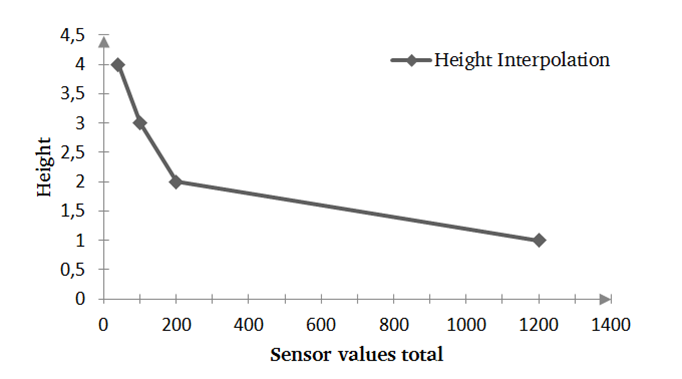
\includegraphics[width=0.6\textwidth]{images/magicbox_data_zaxis}
\caption{Piecewise linear hand distance estimation \cite{Braun2011MultiInputDevice}}
\label{fig:magicbox_data_zaxis}
\end{figure}

Gesture recognition can comprise a large number of different body movements, including sign language that uses movements and position of hands and fingers, the posture of the whole body, or as in our case the movement of the hand in three dimensions. This requires two distinct processing steps. At first it is necessary to precisely localize the position of the hand in the interaction space. Afterwards, a time series of theses positions has to be analyzed and attributed to different gestures. The localization method was first presented in a publication from 2011 \cite{Braun2011MultiInputDevice}. The static gesture recognition method used there was later extended by adapting algorithms used to detect mouse gestures for movements in three dimensions \cite{braun2013capacitive}. 
The first data processing step is the planar localization of the hand, following a weighted average algorithm, whereas $n$ is the number of sensors, $(x_i, y_i)$ the location of the electrode centers and $v_i$ the value of the given sensor.
\begin{align}
\overline{x}&=\frac{\sum^n_{i=1}{v_i\cdot x_i}}{\sum^n_{i=1}{v_i}} & \overline{y}&=\frac{\sum^n_{i=1}{v_i\cdot y_i}}{\sum^n_{i=1}{v_i}}
\end{align}
In order to calculate the distance of the hand from the plane, piecewise linear interpolation is used that resembles the response curve of a single sensor \cite{Braun2011MultiInputDevice}. In this case four different thresholds $t_i$ are used to calculate the proximity, based on the sum of sensor values. $t_1$ indicates the closest distinguishable proximity, e.g. touch, with all higher value sums associated to this. $t_4$ represents the maximum distance in which the sensors can detect a hand. One example with fixed points at values 40, 100, 200 and 1200 is shown in Figure \ref{fig:magicbox_data_zaxis}.

\begin{figure}[h]
\centering
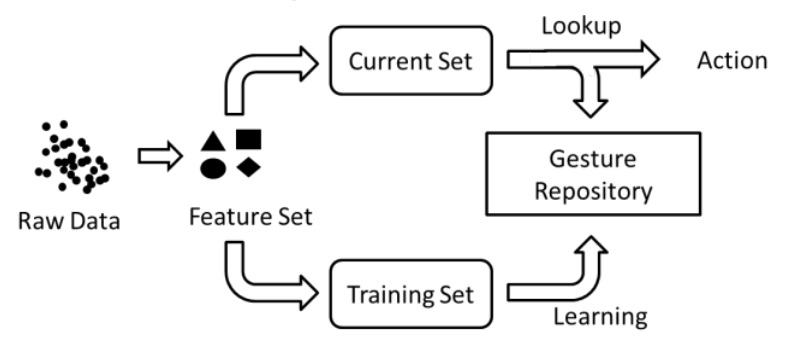
\includegraphics[width=0.7\textwidth]{images/gesture_by_example}
\caption{Principle components of a learning by example recognition framework \cite{braun2013capacitive}}
\label{fig:gesture_by_example}
\end{figure}

Initially a static gesture recognition method was implemented that used a series of five subsequent locations and simple heuristics to determine a small number of gestures. However, this limits the potential gesture set and is difficult to extend. Thus, a generic gesture recognition module was created, based on learning by example \cite{braun2013capacitive}. The general functionality of a gesture recognition framework based on learning by example is shown in Figure \ref{fig:gesture_by_example}. A feature set is extracted from incoming raw data. Collections of these are distinguished into training sets that are used to associate certain features to given gestures. After a learning process the current feature sets that are acquired on-the-fly, are tested against the training sets in a repository. These look-ups can lead to successful gesture recognition and association to certain actions. This association method is also called classification. There are numerous approaches, e.g. neural networks (NN) or support vector machines (SVM).

\subsubsection{Large-area location tracking}
There are several systems that use capacitive proximity sensing to track the location of one or more persons in an environment. A common challenge in large areas is achieving a suitable coverage with electrodes at all positions. Lauterbach et al. overcome this problem in their SensFloor system by integrating sensors and electrodes in an underlay that can be placed below the upper layer of the floor \cite{lauterbach2009}. TileTrack, the system developed by Valtonen et al. requires large emitter electrodes under the floor and receivers placed in the walls \cite{Valtonen2009a}. This limitation was reduced in a later iteration where they integrated receivers into different pieces of furniture.

While SensFloor allows to cover large areas by having the sensing electrodes near all surface areas, a limitation is the maintenance. If a sensor breaks below the floor covering it is difficult to replace. TileTrack in its initial installation requires proximity to walls, or later to specific pieces of furniture that are in the environment. This is difficult to guarantee in many instances and requires an initial calibration of the environment, according to placement of the furniture.

\begin{figure}[h]
\centering
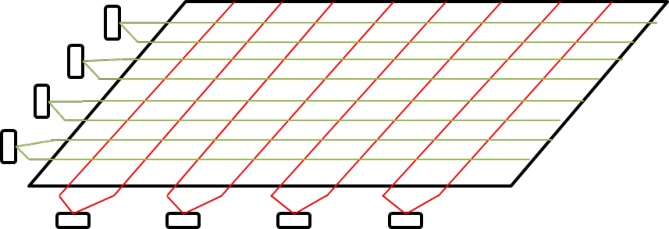
\includegraphics[width=0.8\textwidth]{images/capfloor_concept}
\caption{Wire electrode grid below floor cover attached to sensors on the border}
\label{fig:capfloor_concept}
\end{figure}

I proposed a system based on a rectangular grid of long wire electrodes that are placed below the top floor cover. The sensors are attached at the edge of the area, e.g. in skirting boards \cite{Braun2012CapFloor}. As the system is based on loading mode, there is no need for dedicated receivers, but instead it relies solely on the electrodes below the floor. The system is akin to a larger variety of projected capacitive touch screens that are partially also using grid layouts. However, those typically rely on shunt mode measurements \cite{BarrettScreen}. 

\begin{figure}[h]
\centering
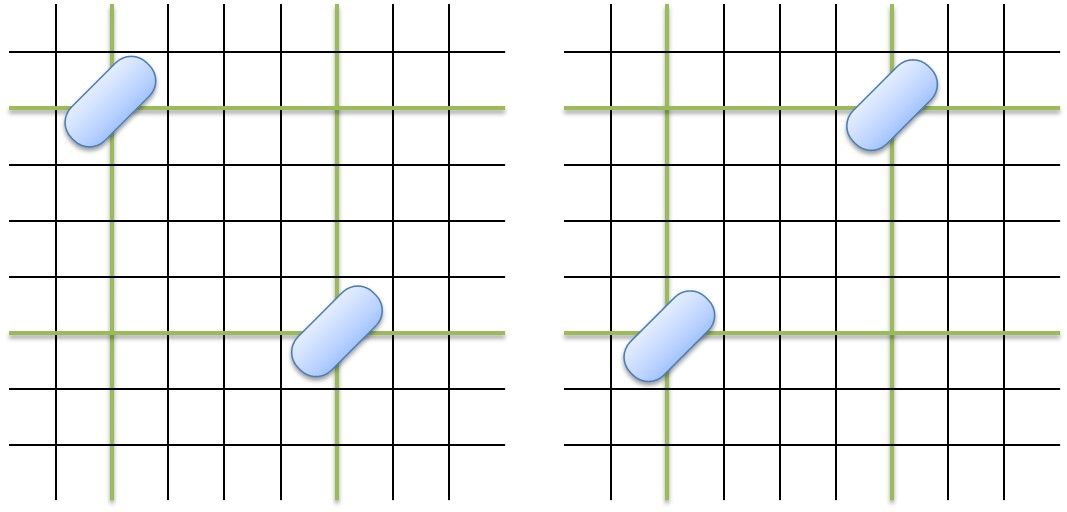
\includegraphics[width=0.8\textwidth]{images/capfloor_ghosting}
\caption{Two potential person locations resulting in same sensor readings (green indicates active electrodes}
\label{fig:capfloor_ghosting}
\end{figure}

Using long, straight wire electrodes has different effects on the measurement. One effect of this is the limited detection distance that is not comparable to large plate electrodes. Particularly if thick floor covers are used, the grid has to be fairly dense. Another effect is the sensitivity towards noise and influence from outside electric fields. Therefore, the system requires preprocessing to reduce the noise and achieve a more robust high-level data processing. In order to localize persons, the system uses an adapted weighted average algorithm, similar to the variety presented for the gesture recognition in the previous section. Each electrode is considered to only have a single coordinate in either $x$ or $y$ direction, allowing to easily calculate the center-of-gravity. However, it can occur that only two electrodes are active at a certain point in time, while two persons are present and too far away from any other electrode to be detected. In these cases there is a certain ambiguity as each $(x,y)$ value combination can result in two potential intersection points, as shown in Figure \ref{fig:capfloor_ghosting}. To overcome this problem, it is possible to either use a mix of sending and receiving electrodes operating in shunt mode and specific measurement cycles, or analyze the time-series of previous locations to discard unlikely positions.

\begin{figure}[h]
\centering
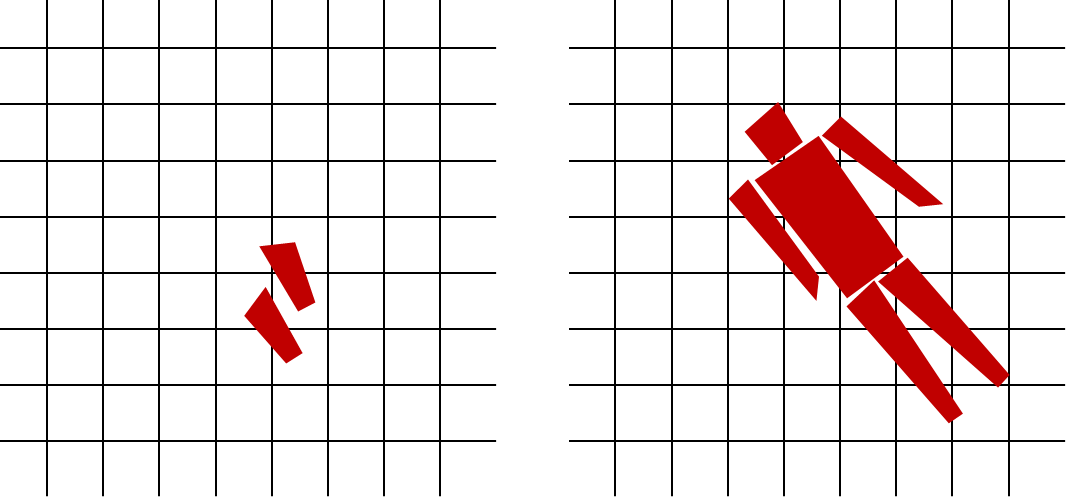
\includegraphics[width=0.8\textwidth]{images/floor_shapes}
\caption{Shapes of a standing and lying person on top of the CapFloor grid}
\label{fig:capfloor_shapes}
\end{figure}

Similar to SensFloor, the concept also supports detecting additional information about the persons present, most notably fall detection. This is based on a time-series analysis of aggregated values of the sensors that are currently detecting an object. This method is using the assumption that the overall sensor response is roughly equivalent to the shape of the object that is closest to the surface. This results in a higher capacitance of the overall system, similar to the plate capacitor model. The effect is shown in Figure \ref{fig:capfloor_shapes}. The sum $s$ of all n sensor values $r$ is the closest equivalent to the system capacitance and therefore a viable measure. If the overall value is beyond a certain threshold $v_l$, we can consider a lying person $p_l$.
\begin{align}
s&=\sum^n_{i=0}{r_i} & p_l&=\left\{ \begin{array}{c}
1,\ \ \ s\ge v_l \\ 
0,\ \ \ s<v_l \end{array}
\right.
\end{align}
In order to increase the robustness this threshold has to be exceeded for a certain amount of time $t_m$. In consequence a fall $f$ is detected if the following equation is 1.
\begin{equation}
f=\prod^{t_m}_{j=0}{p_{l,t_j}}
\end{equation}
\subsection{Model-driven fitting methods}
\label{ch:proc_model}
When acquiring sensor data from physical objects it is often difficult or even impossible to analytically describe the resulting value, as there are numerous environmental factors influencing the signal and the properties of the object might not be clearly determined. Considering the human body, there is a mostly unconstrained number of sizes, shapes and biological properties that influence the response to an electric field. Thus, in order to fit sensor outputs to the potential object configurations, simplified models can be used that resemble the actual physical effects and can be described analytically. Regarding capacitance of the human body relative to a single sensor, a common abstraction is a sphere having a diameter close to the height of an average human \cite{seaver1997human}. Models based on a single geometric objects are considered single-body, while connected geometric objects that comprise a single model can be called multi-body. Smith used a model of multiple spheres to approximate arm position and rotation above an array of capacitive proximity sensors \cite{smith1998electric}. Another possibility is adapting the models to a derived physical effect. Harada et al. are using the projected pressure distribution of a virtual skeleton and body model on a flat surface to create a pressure distribution that can be compared to the actual pressure effect generated by an actual human body resting on a set of sensors \cite{harada2000human}. In this section I will describe two novel methods to fit abstracted models of the human body to sensor readings acquired from smart furniture systems. The first method uses a cylindrical human body model to match the posture of one or two bodies on a bed, the second method uses a multi-body skeleton that is fitted to sensor readings determining posture on a chair.
\subsubsection{Single-body models}
\begin{minipage}{\linewidth}
\centering
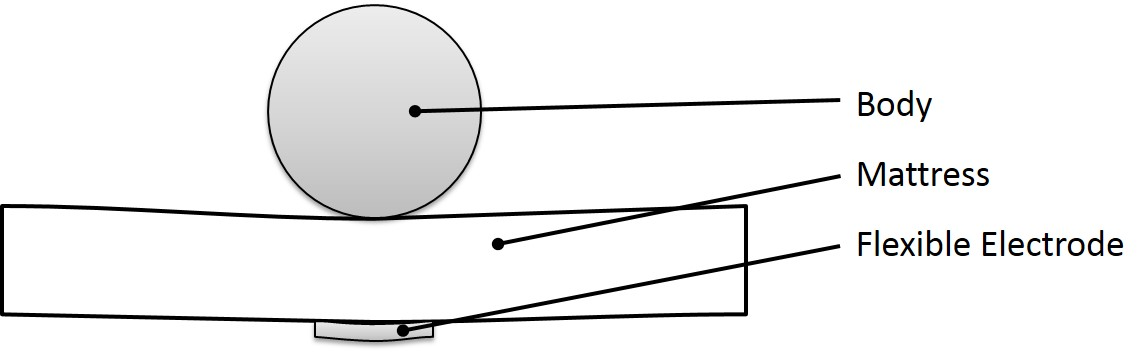
\includegraphics[width=0.8\textwidth]{images/proc_hetero_flexpressure}
\captionof{figure}{Object on mattress decreases distance and changes geometry of flexible electrode \cite{braun2012context}}
\label{fig:proc_hetero_flexpressure}
\end{minipage}

While models are more often applied directly to the capacitive sensor data, it is also possible to use a different property that is derived from it. Together with Henning Heggen, I developed a system that uses flexible electrodes that bend on pressure. In previous experiments we observed that bending a calibrated flexible electrode results in a higher value of the sensor. Thus, the idea was created to use this effect for combining presence and pressure detection. A first application was to use such a system on the slatted frame of a bed \cite{braun2012context}. The following section is based on two different publications \cite{Hamisu2010,braun2012context}. If an object is applying force to the mattress there are two cumulative effects. The object will be in detection range of the sensors, decreasing the distance by deforming the mattress and the applied pressure changes the geometry of the flexible electrode, resulting in a higher sensor value. The basic idea is shown in Figure \ref{fig:proc_hetero_flexpressure}. If a model is used that approaches the pressure distribution of a human body, a small number of capacitive proximity sensors equipped with flexible electrodes should allow to detect different posture and occupation configurations on the bed, including distinguishing sitting and lying, as well as one or two present persons. While the sensor values are increasing according to higher pressure, this relationship is highly non-linear and influenced by three groups of system parameters The sensor system parameters include the sensor design, e.g. excitation voltage and frequency, as well as geometry and material of the electrode. These parameters additionally determine range and precision of the overall system. The second group are environmental parameters that influence the conductivity of the excited electric field, including humidity and temperature. The third group are the bed parameters. These include the hardness of the slatted frame that influences the geometric deformation of the affixed electrodes and the mattress parameters, comprised of hardness, thickness, material and type, influencing how far the body is away from the electrodes and how the pressure is distributed onto the slatted frame.

\begin{minipage}{\linewidth}
\centering
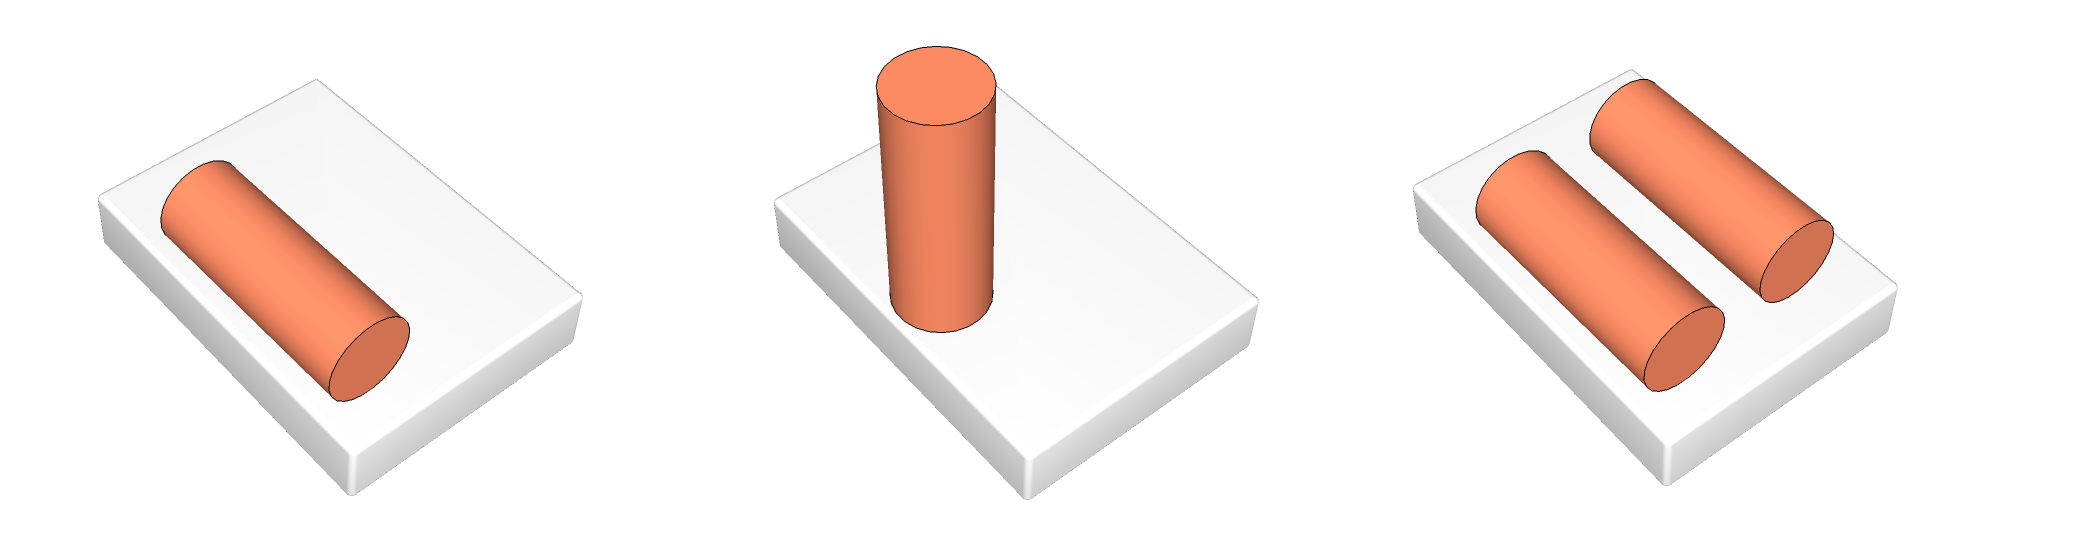
\includegraphics[width=0.8\textwidth]{images/prot_model_bed}
\captionof{figure}{Cylindrical human body model and various poses on mattress \cite{braun2012context}}
\label{fig:prot_model_bed}
\end{minipage}

To identify occupation and positioning we use a very simple model for estimating the effect of a human body on the sensor values. As previously mentioned, the sensors react to both presence of a body and applied pressure. The human body is modeled as a cylindrical object on the mattress. The object can be either sitting or lying and there might be multiple on a single bed. A few potential poses are shown in Figure \ref{fig:prot_model_bed}. It is assumed that a sitting person will cause a high pressure within a small region and that a lying person has a moderate pressure distributed over a larger area. Thus, the challenge of determining posture and orientation from a limited number of capacitive sensors, tuned to detect pressure, can be formulated as an inverse problem. If we assume a constant density of the cylinder and a uniformly deforming mattress, the idealized pressure distribution is uniform as shown in Figure \ref{fig:prot_model_pressure}.

\begin{minipage}{\linewidth}
\centering
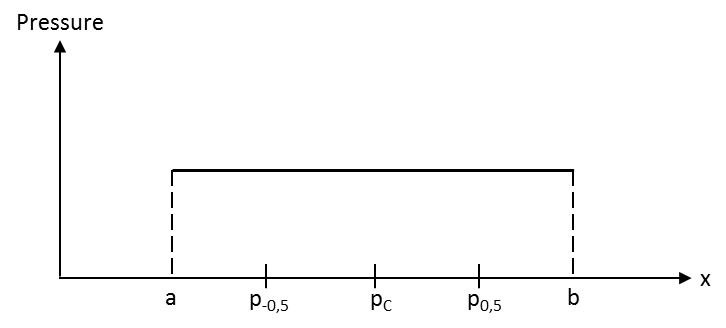
\includegraphics[width=0.6\textwidth]{images/prot_model_pressure}
\captionof{figure}{Pressure distribution of a uniform cylinder \cite{braun2012context}}
\label{fig:prot_model_pressure}
\end{minipage}

The system is further simplified by reducing the significant values of the pressure distribution to just two distinct values. Be $p_c$ is the center of pressure and $p_{-0.5}$, $p_{0.5}$ the points enclosing half of the pressure distribution. The center of pressure and standard deviation $\sigma$ are sufficient to describe the system, as shown in the following equations:

\begin{align}
p_c&=\frac{a+b}{2} & \sigma&=\sqrt{\frac{(b-a)^2}{12}}
\end{align}
\begin{align}
p_{-0.5}&=p_c-\sigma &	p_{0.5}&=p_C+\sigma
\end{align}

The raw data from the sensor is considered as random, uniform sampling, a discretization of the continuous distribution. The center of pressure and the standard deviation are calculated using the geometric information, the position of the sensor $\overrightarrow{x}$.
\begin{equation}
p_c=\frac{\sum_{i=1}^n{v_i\overrightarrow{x}}}{\sum_{i=1}^n{v_i}}
\end{equation}
\begin{equation}
\sigma=\sqrt{\frac{1}{n}(\sum_{i=1}^n{\overrightarrow{x}^2}-\frac{1}{n}(\sum_{i=1}^n{\overrightarrow{x}})^2}
\end{equation}

Using this model a set of potential poses cover the most common situations has been determined. Potential poses for one and two occupants are distinguished. One person may sit at a certain location or lie on the bed in various angles. It is assumed that the head is always at the upper part of the bed. Two persons may either both sit, both lie down, or one is sitting while the other is lying. 
The limitations of this model concerning the actual system are the non-uniform pressure propagation throughout the mattress, as well as the non-linear sensor response on different pressure levels. Therefore, it is not expected that the deviations adhere to the theoretical model, but instead configurable thresholds are used that allow for increased robustness in exchange for precision.

\begin{minipage}{\linewidth}
\centering

\includegraphics[width=0.7\textwidth]{images/smartbed_cog}
\captionof{figure}{Calculating centers of pressures and deviation \cite{braun2012context}}
\label{fig:smartbed_cog}
\end{minipage}

Occupation and posture detection are performed by dividing the two person bed into a left and right section. For each side the total sensor values, assumed center of pressure using weighted average and the standard deviation are calculated individually(Figure \ref{fig:smartbed_cog}). The same calculation is performed between the two areas, allowing to distinguish the specific side of activity or detecting persons that are lying on the bed diagonally.
Using these six intermediate values it is possible to map the different poses. If all activity is on one side and the horizontal deviation is low, it can be assumed that one person is sitting. Additionally, the intermediate values can be used to gather more information, e.g. the exact location a person is sitting at. 

\subsubsection{Multi-body models}
If it necessary to identify more complex human behaviors than sitting and lying, a single body model is no longer sufficient. In the briefly mentioned work by Harada et al. the underlying model was a 3D representation of an average human body that could move various joints freely \cite{harada2000human}. This allows to detect a variety of different postures, in this case using an iterative process based on potential energy, momentum and difference between the actual and simulated pressure distribution. Using such full body models, based on an internal skeleton of connected joints is also common in full body gesture tracking systems. However, while in those cases the volume of the different body parts is important, there is not necessarily any additional physical simulation of properties, such as weight and density \cite{Shotton2013}. 

In a project together with student Sebastian Frank, a concept for a smart chair was developed that unobtrusively integrates a set of capacitive proximity sensors to detect presence, posture, activity and breathing rate of a person sitting on the chair \cite{Braun2013ChairAid}. By placing suitably sized electrodes strategically, at locations that allow getting a good measure of the most significant body parts. Using eight electrodes distributed between seat, backrest and armrests it the sensor values are mapped to postures using two different methods, according to the specific purpose of the underlying application. The first method directly translates the sensor values to body part positions, while the second uses a machine learning classification.

\subsubsection*{Direct manipulation of skeleton model}
\begin{minipage}{\linewidth}
\centering
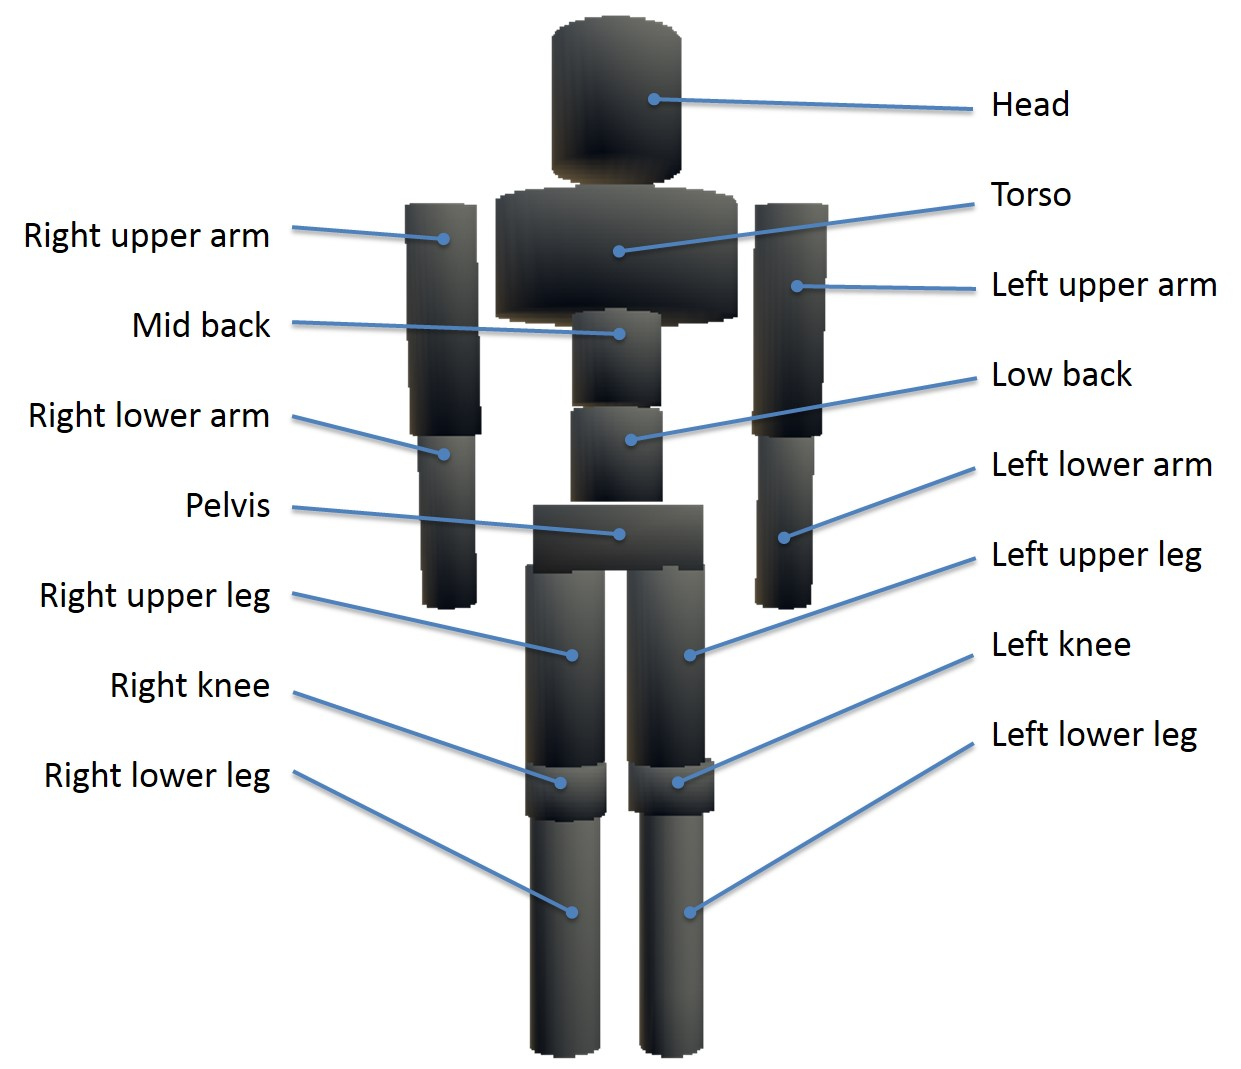
\includegraphics[width=0.8\textwidth]{images/smartchair_skeleton_model}
\captionof{figure}{Smartchair skeleton model and associated body parts}
\label{fig:smartchair_skeleton_model}
\end{minipage}

In Figure \ref{fig:smartchair_skeleton_model} the skeleton model can be seen. The skeleton model is comprised of 15 different groups. As those are combined to each other the degrees of freedom are significantly reduced to just 10. Sensors close to the different body parts will modify the associated parts of the model. As an example, the distance of the left lower arm group is determined by the sensor in the left armrest. However, as the groups are connected, this will also modify the orientation of the left upper arm. Accordingly, if the sensor behind in the lower backrest detects a receding lower back, the position and orientation of the other back groups, head and arms are also modified. Thus, the fitting method attempts to place the different groups of the model according to current sensor readings. A collection of rules is used that follows the flowchart outlined in Figure \ref{fig:capchair_flow}.

\begin{minipage}{\linewidth}
\centering
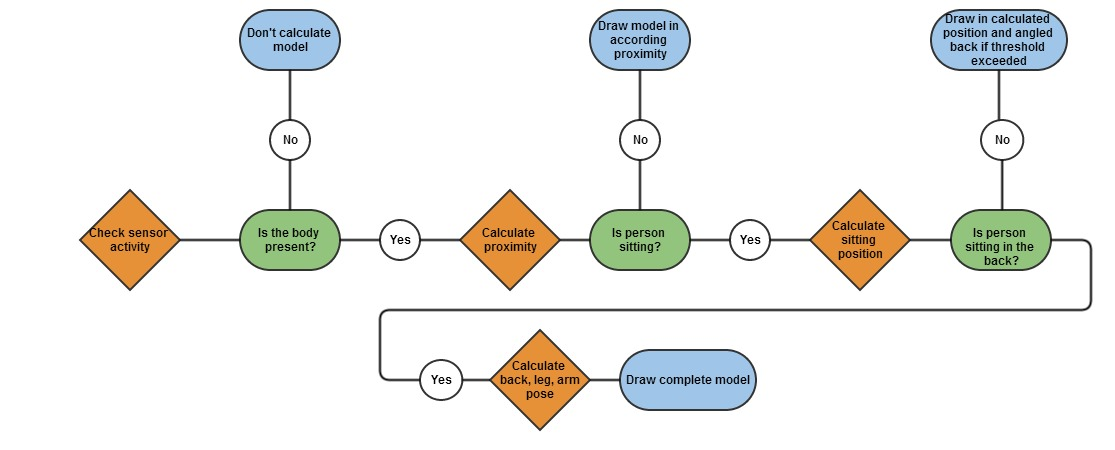
\includegraphics[width=0.9\textwidth]{images/capchair_flow}
\captionof{figure}{Flowchart of the model fitting process of the grouped skeleton parts and performed calculations}
\label{fig:capchair_flow}
\end{minipage}

The calculation of the different steps varies and is outlined shortly in the following enumeration:
\begin{enumerate}
\item \emph{Check sensor activity} uses a threshold of the different sensors to determine the presence of any objects in detection distance
\item \emph{Calculate proximity} use a second thresholds of seat sensors to determine sitting or non-sitting status
\item \emph{Calculate sitting position} use a weighted average of the seat area sensors to determine position on seat
\item \emph{Calculate back, leg, arm pose} calculate back pose by determining distance from back to backrest based on sensor values. Raise leg according to proximity to front seat sensor. Calculate arms based on proximity to arm rests.
\end{enumerate}

This method allows a fine-grained fitting of the model to the sensor values that closely resembles the pictures of a person moving in the chair. A number of poses and the accordingly fitted 3D models using this method can be seen in Figure \ref{fig:smartchair_skeleton_poses}.

Using a fitting method that allows to detect fine movements enables a number of unique applications. One example is to track a set of different exercises that can be performed on an office chair, in order to prevent future back problems. Following an exercise routine can significantly reduce the indicative risks \cite{robertson2009effects}. Some of the common exercises can be tracked for accuracy and number of repetitions using the capacitive proximity sensors in the chair.

\begin{minipage}{\linewidth}
\centering
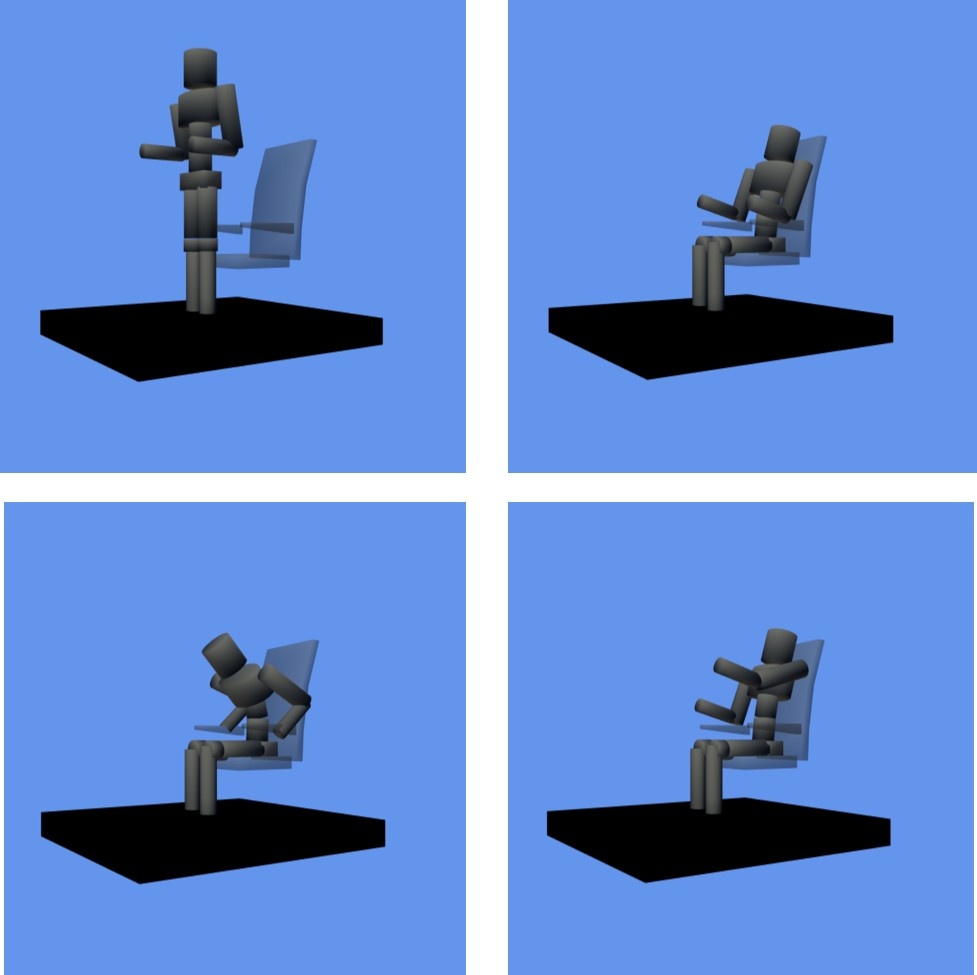
\includegraphics[width=0.7\textwidth]{images/smartchair_skeleton_poses}
\captionof{figure}{Screenshots of the Capacitive Chair application showing different poses of the skeleton model}
\label{fig:smartchair_skeleton_poses}
\end{minipage}

A limitation of the above method are the fixed threshold levels that are set based on experience. Either a calibration method can be used that personalizes the different thresholds, or another form of classifications that is based on training with a larger variety of different body volumes. It is suitable to use machine learning methods for this task, as they are designed to learn from a larger set of training data and provide numerous classification methods. However, this leads only to a discrete set of different postures, limiting some potential applications. One potential method is described in the following section.

\subsubsection*{SVM classification}
\begin{minipage}{\linewidth}
\centering
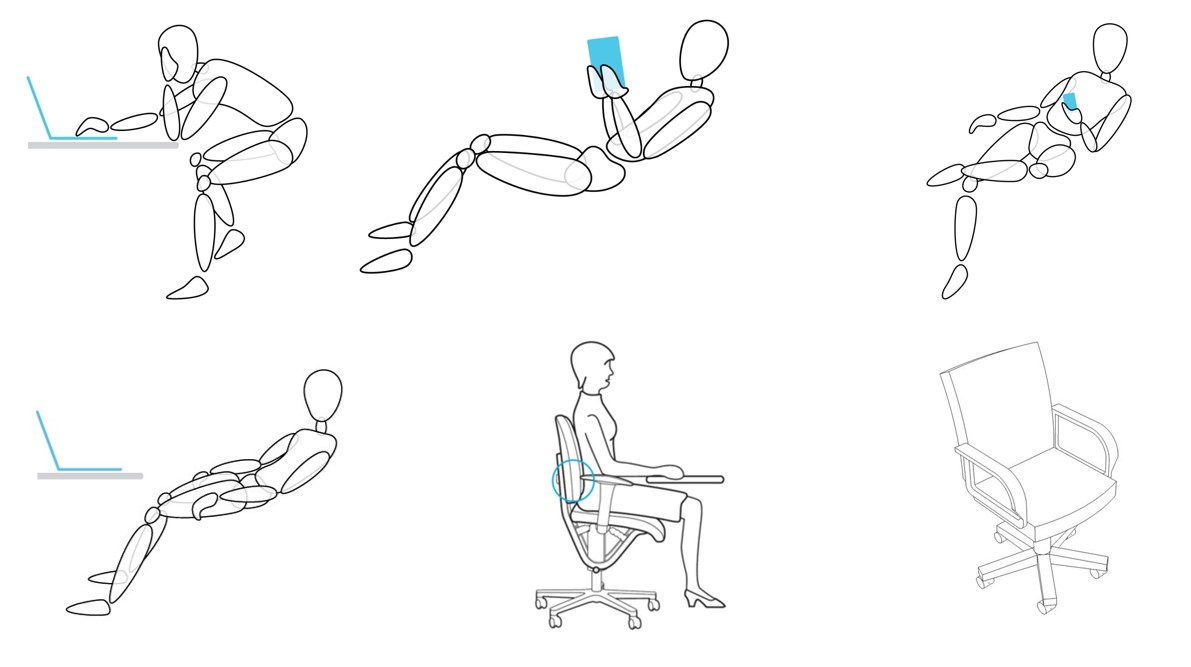
\includegraphics[width=0.7\textwidth]{images/smartchair_gps_poses}
\captionof{figure}{Selected set of postures from Global Posture study and own gestures. \emph{From top left to bottom right:} The strunch, the draw, the smart lean, the take it in, upright, no person (first four taken from \cite{globalPosture}}
\label{fig:smartchair_gps_poses}
\end{minipage}

Support vector machines (SVM) are a supervised learning method that is primarily used for linear classification of n-dimensional features \cite{hearst1998support}. They are clustering data by calculating a hyperplane from training data that maximizes the distance from the closest features. A fast learning method is using sequential minimal optimization and was proposed by Platt \cite{platt1999fast}. The algorithm requires normalized values. A dynamic normalization algorithm constantly analyzes the sensor data for minimum and maximum values and accordingly calculates the normalized value. There is a variety of different software frameworks for machine learning that support training and recall of SVMs, thus there is no need for reimplementing these methods. As there is an implicit weighting of features according to significance, there is no need to pre-process or weigh the sensor data.

The training data is collected from a set of persons that have a significant variance in body shapes in both height and girth. SVMs support an arbitrary number of different groups for classification. However, the number of significant poses on a chair is limited. The Global Posture Study by office furniture manufacturer Steelcase Inc. analyzes the most common poses with a focus on information consumption from modern technical devices, such as smart phones or tablets \cite{globalPosture}. The different postures are shown in Figure \ref{fig:smartchair_gps_poses}. A capacitive office chair should be able to distinguish most of these poses if training data has been collected from a large enough number of suitable candidates. Additionally, using sensors clearly positioned on a certain side of the chair, e.g. the armrest sensors, it is possible to associate directional varieties of the asymmetric postures.
\subsection{Heterogeneous sensor systems}
Heterogeneous sensor systems have been an active research topic in the last decades. They can be described as a collection of sensors in the same domain that are measuring different physical properties or the same properties using different methods \cite{buczak1998self}. The majority of research is aimed to enable a self-organization of networks of heterogeneous sensors, or combine the data of heterogeneous sensors in a meaningful fashion. For capacitive proximity sensors another factor of heterogeneity has to be considered - the vastly flexible shape and material of the electrodes. This allows to create ensembles of capacitive sensors in a single domain that serve different purposes, e.g. large electrode sensors that detect the presence of a body over a longer distance combined with small electrode sensors in a specific area to detect touches. The more traditional approach combines the data generated by different categories of sensors in a meaningful fashion, to create higher level information that would not be available otherwise. One example of this approach is the previously presented LaZMouse by Smith, that added palm proximity sensing to a typical computer mouse \cite{smith1999thesis}.

In this section I will present two different contributions. The first is a concept for a heterogeneous capacitive sensor array that combines large electrode sensors to detect the presence and configuration of limbs and numerous densely packed small electrodes enabling gestural finger interaction. The second system aims at alleviating the inability of capacitive proximity sensors to clearly identify touches if the electrodes are at a distance from the touch surface. Data acquired from a microphone listening for the acoustic effects of a finger touching the surface are combined with capacitive proximity sensor data, to combine mid-air interaction and touch recognition.
\subsubsection{Heterogeneous capacitive arrays}

\begin{minipage}{\linewidth}
\centering
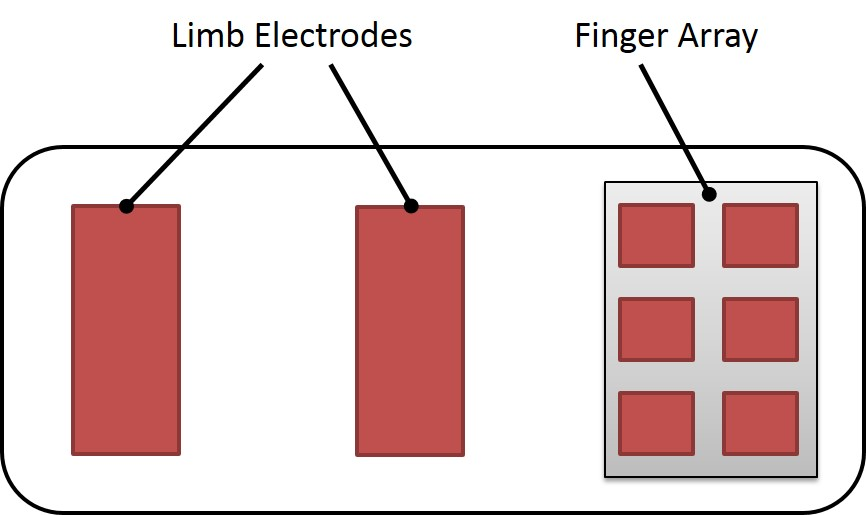
\includegraphics[width=0.7\textwidth]{images/proc_hetero_array}
\captionof{figure}{Heterogeneous sensor array for limb detection and finger tracking}
\label{fig:proc_hetero_array}
\end{minipage}

An often-cited issue of mid-air interaction systems is discriminating between an intended gesture and arbitrary movements in the detection area \cite{hinckley1994survey}. While traditionally used for full-body gesture systems, this is also true for capacitive proximity sensors that provide 3D tracking. If the interactive zones are to be integrated in design features that serve multiple purposes, there need to be methods that distinguish between typical use and intended interaction. In a project with students Sönke Schmidt and Stephan Neumann I developed a concept for a car armrest equipped with a capacitive finger interaction system \cite{braun2013ActiveArmrest}. A regular car armrest is augmented in a way that integrates the capacitive sensors in an invisible fashion. In this case it is necessary to clearly distinguish between intended control gestures by the driver or if he is just resting the arm. The idea is to use the status of both arm and hand to identify the intention. The system is using a heterogeneous combination of capacitive proximity sensors. Sensors in the middle and back of the armrest are used to detect the current status of the arm, while an array of smaller electrodes in the front can track a variety of finger gestures. The setup is shown in Figure \ref{fig:proc_hetero_array}. 

\begin{minipage}{\linewidth}
\centering
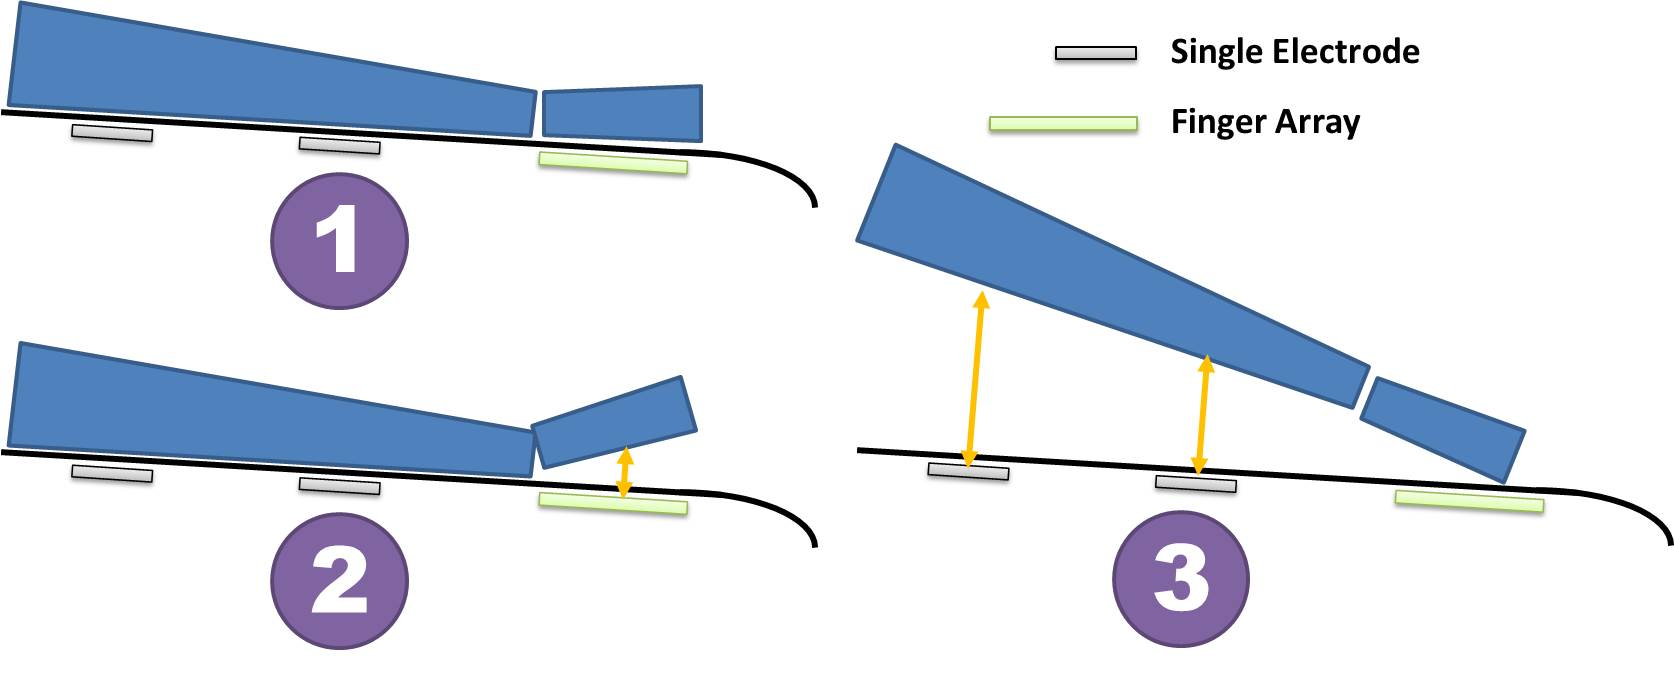
\includegraphics[width=0.8\textwidth]{images/proc_hetero_postures}
\captionof{figure}{Arm model and detection of posture based on distances to two sensors and finger array for resting position (1), hand raised position (2) and arm raised position (3)}
\label{fig:proc_hetero_postures}
\end{minipage}

In Figure \ref{fig:proc_hetero_postures} three different positions are shown that arm and hand can have on the armrest. 
\begin{enumerate}
\item Arm and hand are in resting position with both close to the surface
\item Arm resting on the back and the hand hovering in proximity of the front area
\item Arm raised position and fingers touching the front of the armrest
\end{enumerate}
The latter two positions are suitable for finger-based gestural interaction as they can be moved freely. The system should therefore be able to distinguish between the three different positions and consider either position (2) or (3) or both as intended interaction. Different interaction patterns have to be chosen for both active positions. Regarding the arm raised position the person will typically want to interact using familiar touch gestures. In the hand raised position it is necessary to track gestures that are performed in the air. In both cases we assume that a single finger is used. A set of four different gestures has been defined for both interaction methods. The number is sufficient to control the user interface that we have developed and support both navigation and selection. The type of gestures has been defined after looking at previous research into touch and hand gestures \cite{bragdon2011experimental, wachs2011vision}. For the touch interaction left and right swipes performed with either one or multiple fingers are supported. Regarding the free-air interaction we are using left and right swipes, as well as planar circles either clockwise or counter-clockwise. 
 
The data processing of the system therefore requires three distinct steps. At first the three specified limb postures have to be identified. Afterwards, the position of the fingers in or above the interaction area have to be calculated, and finally a time-series analysis of subsequent positions has to be performed, in order to infer different gestures. The two distinct arm sensors are able to determine single distance values. In addition the aggregated data of the finger detection array in the front is used to detect a third distance value. To map the different postures, a set of thresholds is used that determine if arm or hand are touching the armrest surface, or if they are hovering above it. Be $r_b$ the value of the sensor in the back, $r_m$ the value of the sensor in the middle and $r_f$ the aggregated value of the sensor values in the front $r_{f,i}$. Using three threshold levels $t_b$, $t_m$ and $t_f$ the different postures $p\epsilon{1,2,3}$ can be determined as follows
\begin{align}
r_f&=\sum^n_{i=0}{r_{f,i}} & p&=\left\{ \begin{array}{c}
1,\ \ \ r_b\ge t_b \wedge r_m\ge t_m \wedge r_f\ge t_f\\ 
2,\ \ \ r_b\ge t_b \wedge r_m\ge t_m \wedge r_f< t_f \\ 
3,\ \ \ r_b< t_b \wedge r_m< t_m \wedge r_f\ge t_f \end{array}
\right.
\end{align}
As we are acquiring sensor data proportional to distance it is also possible to calculate orientation angles of the arm and use it as input. However, for now this was not followed up any further.
The calculation of the finger position in three dimensions is adapted from the previously introduced method for sparse capacitive arrays to track objects in three dimensions that uses a combination of weighted average for planar location and stepwise linear interpolation to determine the height. 

To classify the gestures we are using points from a distinct start to a distinct stop. In case of the free-air interaction this is determined by the finger moving in a constrained part of the interactive area. In case of the touch interaction it is determined  by a finger starting and stopping to move, while exceeding a threshold indicating touch. The points between start and stop position are normalized and we are using a SVM classifier to detect the trained gestures. There are distinct classifiers for the two different methods that are triggered according to the selected interaction pattern. The SVM is trained using the sequential minimal optimization method by Platt \cite{platt1999fast}.

\subsubsection{Heterogeneous sensor fusion}
\begin{minipage}{\linewidth}
\centering
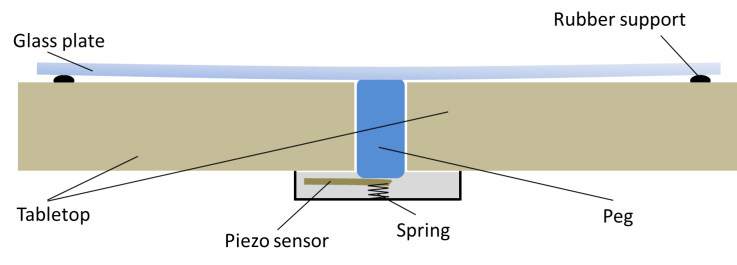
\includegraphics[width=0.8\textwidth]{images/captap_peg}
\captionof{figure}{Suspended peg knock detection system}
\label{fig:captap_peg}
\end{minipage}

As previously mentioned capacitive proximity sensors inherently lack the ability to detect touches if the electrode is at a distance from the touch surface. This may be overcome easily in systems that are tuned to work in close proximity, e.g. SmartSkin \cite{rekimoto2002smartskin}. Another option is adding a different sensor category specifically for detecting touches. The pressure applied to the surface can be detected by a suitable sensor, e.g. by using a surface suspended on sensors, such as the weight-aware dining table by Chang et al. \cite{chang2006diet}. However, this requires a specific construction and can't be retrofitted to existing systems. Additionally, there are restrictions to the potential rigidity. A different effect of surface touches is the acoustic response. A microphone connected to the surface can detect a variety of different touch events. Harrison et al. presented a system that detects varieties of fingernail scratches performed on a rough surface \cite{harrison2008scratch}. The system was later extended to detect impact events by different parts of a finger or pens \cite{harrison2011tapsense}. 

In collaboration with Sebastian Zander-Walz and Stefan Krepp I have tested different methods to combine sensors for dedicated touch detection and capacitive hand tracking integrated into an existing living room table, thus providing a potential to retrofit existing pieces of furniture \cite{Braun2013captap}. A first idea was to use a single piezo sensor to detect vibration of a glass plate that covers a living room table. The concept is shown in Figure \ref{fig:captap_peg}. This first system was prone to outside influence and had difficulties detecting multiple touch events. The second iteration used a microphone system similar to the concept provided by Harrison. However, it was extended to distinguish both impact events and different swipe varieties in a single module. The basic idea is to analyze the acquired acoustic signals in the frequency domain and use a classification method based on a number of selected features related to frequency. The supported gestures and the associated FFT profiles are shown in Figure \ref{fig:alltouch}.

\begin{minipage}{\linewidth}
\centering
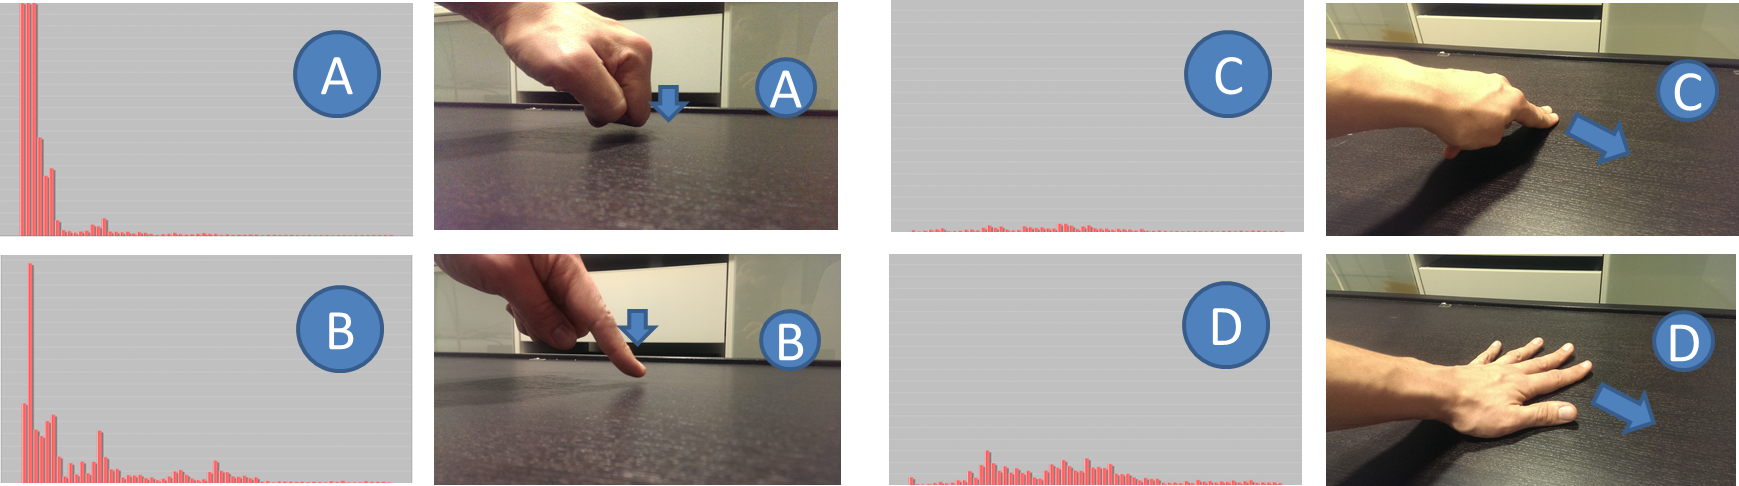
\includegraphics[width=1.0\textwidth]{images/alltouch}
\captionof{figure}{64 sample FFTs and photo for a knock event (A), a finger tap (B), a finger swipe (C) and a hand swipe (D)}
\label{fig:alltouch}
\end{minipage}

At first the audio signal is acquired using a 96kHz sample rate and a feature extraction rate of 375Hz (using a  Hanning type sliding window of 4096 (and 256 samples overlapping) samples per extraction. In order to perform a classification over this signal a variety of different features are considered. The signal differences are most significant in the frequency domain, thus we are performing a FFT over 4096 samples, looking at the first 512 of 2048 magnitude values, thus covering the frequency range up to 12kHz. We are collecting the mean value, the standard deviation and the index of the highest value within the frequency range. This process is repeated for a downsampled FFT of 64 values, similar to the method used by Harrison et al. Another frequency domain-feature we are using is the centroid, i.e. the weighted mean of the present frequencies. Additionally, we are using two time-domain features, the RMS power (root mean square), i.e. the average magnitude within the current frequency band and the number of zero crossings of the signal.

\begin{minipage}{\linewidth}
\centering
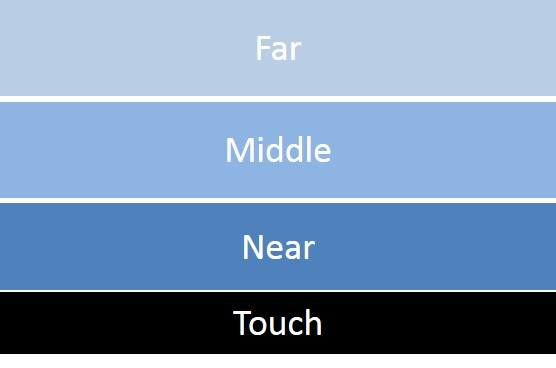
\includegraphics[width=0.5\textwidth]{images/captap_layer_interaction}
\captionof{figure}{Multiple interaction layers}
\label{fig:captap_layer_interaction}
\end{minipage}

As previously mentioned there are several limitations of free-air gesture interaction systems, related to user fatigue \cite{Baudel1993,lenman2002}. Additionally, the achievable resolution of the area above the surface of the capacitive proximity sensors is considerably lower than on the plane. If these two aspects are combined, an interaction pattern that includes a tactile sensation for improving selection events in graphical user interfaces and a sparse quantization of the interaction space above the surface seems viable. Thus we are proposing a layer-based interaction for capacitive proximity sensor devices that is comprised of a touch layer that can be used to register several different types of touch events and three different distance layers based on the proximity of the hand \cite{Braun2013captap}. This is inspired by similar multi-layer patterns introduced by Subramanian et al. for pen-supporting tabletop interaction systems \cite{subramanian2006multi}. The different layers in Figure \ref{fig:captap_layer_interaction} are intended for touch and free-air interaction. The touch layer at the bottom of the Figure represents the interaction on the surface of the table. The layers on top are formed by dividing the area above the table in three equally large parts – the near layer, the middle layer and the far layer, realized using the elevation calculation presented in the algorithm section. Inside each layer a set of different gestures can be executed and recognized while inter-layer changes may trigger additional events. Different interaction types are used for the touch and the free-air gesture layers. Swiping and dwelling gestures are suited for the free-air gesture layers while at the touch layer tapping, double tapping and different swiping patterns can be used. These interaction types may have at each layer a different functionality.

\subsection{Image-based processing}
Their ability to detect changes in the electric field over a distance has led to capacitive proximity being regarded as similar to cameras. Smith et al. consequently called their approach electric field imaging, as particularly shunt mode measurements and their constrained electric fields allow applying certain image processing methods, e.g. tomography \cite{Smith1999a}. They were critical of using similar methods for shunt mode, noting the following statement.
\begin{quote}
Loading mode measurements can be likened
to images formed without a lens, since only one "end" of
each field line is constrained by the measurement. \cite{smith1998electric}
\end{quote}
Nonetheless, loading mode has certain advantages, particularly if all electrodes are in a single plane and we would like to have a higher sensitivity at a distance from the plane it is advantageous if there is no receiving potential nearby. One example for this planar electrode setup is large area gesture interaction devices, e.g. a table that is able to track the position of arms and hands in three dimensions. There is a plethora of image-based object detection and tracking algorithms that can be also used for capacitive proximity sensor data processing. There is a short process that I propose to realize this arm and hand tracking that includes some general steps that can be used to identify a variety of objects. The process is distinguished into four distinct steps:
\begin{itemize}
\item Creating a grayscale image from the acquired sensor data
\item Apply a feature-preserving image upscaling method
\item Find the contours of the present objects according to pixel values
\item Analyze the image moments of the contour areas and fit human arms
\end{itemize} 

\begin{figure}[h]
\centering

\includegraphics[width=0.5\textwidth]{images/proc_im_pixels}
\caption{Pixel array mapped from sensor values}
\label{fig:proc_im_pixels}
\end{figure}

The most challenging aspect of the first step is the low resolution of a reconstructed image. In order to achieve a mid-range distance resolution that allows detecting objects within 30 or 40 cm it is necessary to use electrodes that are sufficiently large. Thus, an example device uses an array of 6x4 sensor electrodes, resulting in an image of only 24 pixels. Typically the sensor values are an integer value in a range between 0 and 15000. Accordingly we can create a single-channel image with a channel depth of two bytes. In our case we use a linear mapping of sensor values to pixel intensities. An exemplary result image of this mapping is shown in \ref{fig:proc_im_pixels} (with enlarged pixels). In this format it is difficult to gather information about the exact position of the arms and thus we need to apply further processing before finding the contours and fitting arm objects.
\begin{figure}[h]
\centering
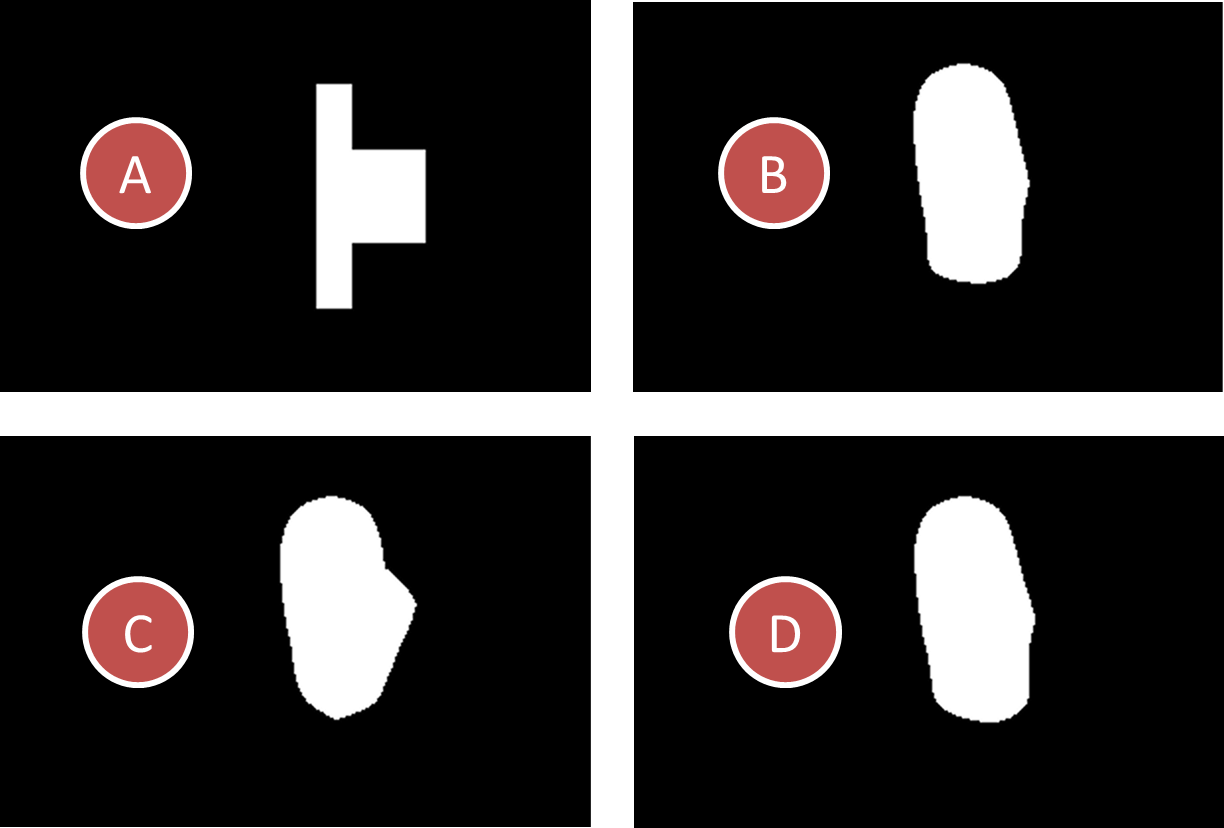
\includegraphics[width=0.9\textwidth]{images/proc_im_interpol}
\caption{Effect of different upscaling methods on shape, (A) nearest neighbor, (B) bicubic, (C) bilinear, (D) Lanczos4 - shown as thresholded binary images (pixel intensity > 30)}
\label{fig:proc_im_interpol}
\end{figure}

\subsubsection{Acquire and optimize contours}
In order to get the relevant contours of objects in the interaction area we have to apply some further processing. The first step is to enlarge the image using a feature-preserving scaling method. As all sensors are prone to environmental noise we apply some thresholding based on the pixel intensities before looking for contours. The result is an enlarged binary image of black and white pixels. We have tested four different image scaling methods, nearest neighbor, bilinear interpolation, bicubic interpolation and Lanczos interpolation. Exemplary results are shown in \ref{fig:proc_im_interpol}. The Lanczos interpolation showed the best results but is most processing intensive. However, since we are dealing with small images it is reasonable for CapTap. The contours are calculated based on those binary images, defined as the borders between black and white regions. For further processing we are looking into the distribution and the intensities of the pixels within the specified region.
\begin{figure}[h]
\centering
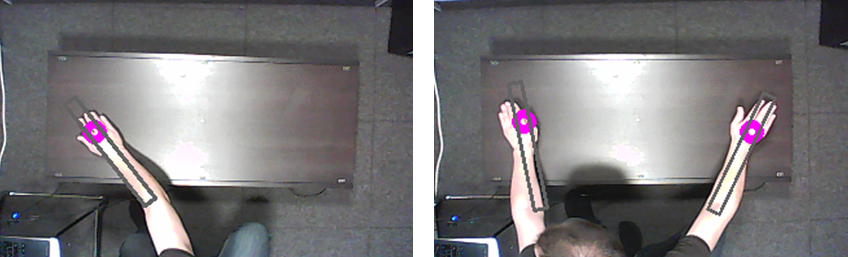
\includegraphics[width=0.9\textwidth]{images/proc_im_arms}
\caption{Overhead camera picture of the scene overlaid with live arm and palm reconstruction for one arm (left) and two arms (right)}
\label{fig:proc_im_arms}
\end{figure}

\subsubsection{Palm and arm fitting}
The last step of identifying and tracking the arms is to fit the position and orientation of the palms and arm into the acquired object contours. For this task we are analyzing the image moments within the contours. These are certain particular weighted averages of pixel intensities, or a function thereof \cite{hu1962visual}. They can be calculated using the following equation, whereas $j$ and $i$ define the order and $I(x,y)$ is the pixel intensity at a given position. We can use this to calculate the center point $(\overline{x},\overline{y})$, leading to the central moments $mu_ji$ that are required to determine the orientation of the contour as angle $\gamma$.
%m_ji=∑_(x,y)▒〖I(x,y) x^j y^i  〗,x ̅=m_10/m_00 ,y ̅=m_01/m_00 
%〖mu〗_ji=∑_(x,y)▒〖I(x,y) (x-x ̅ )^j (y-y ̅ )^i  〗
% γ=0.5∙arctan (2∙〖mu〗_11)/(〖mu〗_20-〖mu〗_02 )
\begin{equation}
m_ji=\sum_{(x,y)}{I(x,y)x^jy^i}
\end{equation}
\begin{equation}
\overline{x}=\frac{m_10}{m_00}, \overline{y}=\frac{m_01}{m_00}
\end{equation}
\begin{equation}
mu_{ji}=\sum_{(x,y)}{I(x,y)(x-\overline{x})^j(y-\overline{y})^i}
\end{equation}
\begin{equation}
\gamma=0.5\cdot arctan\frac{2\cdot{mu_{11}}}{mu_{20}-mu_{02}}
\end{equation}
 
We use the center point and orientation to calculate the estimated position of the palm of the hands. These points are the basis for the subsequent gesture recognition. Additionally, we are using separate Kalman filters for smoothing the different palm positions and arm orientation. The resulting arm reconstruction and the actual arm position in a photo are shown in \ref{fig:proc_im_arms}. We installed a simple webcam above the table and registered the table position to the camera image. 

The arm reconstruction so far is mostly used to determine the arm position. Another potential use of the arm orientation is to improve the merging of two hands. While the system can't distinguish from a single sensor if one hand is close or two hands are further away, we can use the presence of two arms to identify the overall number of objects in the detection range. 
\subsubsection{Intensity-based elevation estimate}
A distinct challenge of the capacitive hand tracking is the considerable directional difference in available resolution. While we can use the presented image analysis to track the planar position of the arms over the whole table area of 80cm width and 50cm depth, estimating the elevation of the arm above the table is restricted by the proximity range of the single sensor. Typically the achievable range maxes out at around 35cm, depending on environmental conditions. In a plate capacitor system the distance $d$ is proportional according to size of the plates $A$ and resulting capacitance $C$. Due to the linear mapping of sensor capacitance measurements to pixel intensities $I$ we can use the image moment within a contour $S$ as estimate of the actual capacitance, and calculate the elevation $e$ according to the following equations:

\begin{align}
d&\propto{\tfrac{C}{A}} & S&\propto{\tfrac{m_{00}}{\int{S}}}
\end{align}

The same thresholds discussed in the contour retrieval phase apply to this step, thus leading to discarding objects at a larger distance that are difficult to detect. Starting from this threshold we normalize the resulting elevation according to a maximum threshold for m00 that denotes a very close object (such as touch). The actual touch recognition is performed using acoustic methods. 
As previously explained the sensors are prone to environmental influences, thus this just allows to get an estimate of the actual elevation and no absolute distance value. Therefore, the interaction should not be designed to require a highly precise discrimination of different elevation values, but instead use more of a 2.5D paradigm. Our take on this will be presented in the application section.
\subsection{Physiological signals in frequency- and time-domain}
\subsubsection{Respiratory rate}
\subsubsection{Sleep phase recognition}
The most reliable way to track sleep phases is by using an electroencephalography (EEG); that is measuring the electrical activity of the brain by placing electrodes on the scalp. Various different types of neural oscillations can be distinguished - the most important for sleep phase detection are alpha waves, theta waves, delta waves and sleep spindles. The American Academy of Sleep Medicine (AASM) distinguishes three different phases of non-rapid eye movement sleep (NREM) and REM phase [11]. 
\begin{itemize}
\item Stage 1 - occurs mostly in the beginning of sleep. It has slow eye movement, alpha waves disappear and the theta wave appears. 
\item Stage 2 - dreaming is very rare and no eye movement occurs. The sleeper is quite easily awakened. EEG recordings have a tendency for characteristic "sleep spindles"
\item Stage 3 - was previously divided into stages 3 and 4. It is slow-wave sleep (SWS) or deep sleep. Stage 3 used to be the transition between stages 2 and 4 where delta waves began to occur, while delta waves are dominant in stage 4. 
\item REM sleep - is a phase of sleep characterized by random and rapid movement of the eyes. It is considered the lightest phase of sleep and occurs all through the night but gets longer close to morning.
\end{itemize}

\begin{minipage}{\linewidth}
\centering
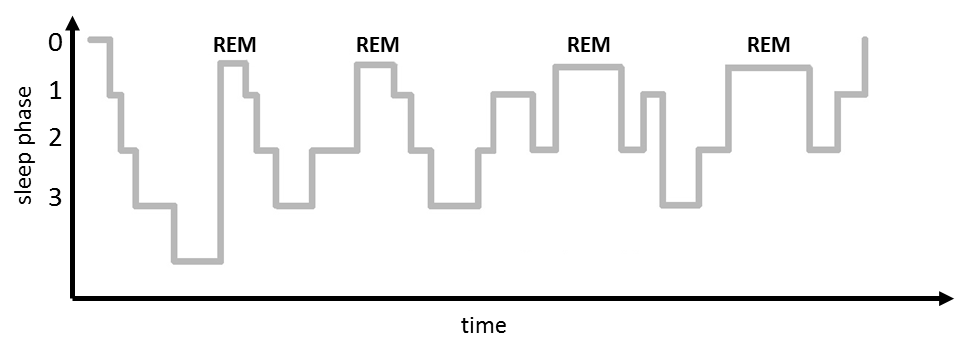
\includegraphics[width=0.6\textwidth]{images/proc_phys_sleepphase}
\captionof{figure}{Example of human sleep phases throughout the night}
\label{fig:proc_phys_sleepphase}
\end{minipage}

A typical distribution of sleep phases throughout the night is shown in Figure \ref{fig:proc_phys_sleepphase}. It can be easily seen that the sleep is distributed into different cycles, whereas the sleeping person is moving through the different sleep phases until having a REM phase and then going back to deep sleep. If the only available data is body movements it is becoming more difficult to reliably determine the sleep phase. Studies have shown that the magnitude of movement is typically associated to the follow-ing phases in decreasing order: wake, stage 1, REM, stage 2, stage 3 [12]. Another method is distinguishing between awake phase, active sleep and quite sleep and takes into account the order of those phases. This information allows to correlate the actual sleep phases with good certainty [13]. We have chosen this method for our system.

Capacitive proximity sensors enable us to detect the presence of suitable object and their relative proximity to the electrode. Consequently a moving object will cause a change of sensor values. If we aggregate these data deviations from an array of sensors we get a reliable measure of objects moving above the electrodes. In the case of MoviBed we can assume that there is a limited number of persons moving on top of the sensors and thus it is possible to associate the sensor values to movement. In the following we will present a suitable method to achieve a reliable detection of the movements of a sleeping person. We are following a similar approach as Salmi and Leinonen [13].
At any given time t a set of the latest values of all n sensors can be stored as a tuple in the following form: 
\begin{equation}
\overrightarrow{s_t}=\begin{pmatrix}
s_{1_t}\\ 
s_{2_t}\\ 
\vdots \\ 
s_{n_t}
\end{pmatrix}
\end{equation} 

%(s_t ) ⃗=(■(s_(1_t )@s_(2_t )@■(⋮@s_(n_t ) )))
As capacitive proximity sensors are particularly susceptible to external influences, such as temperature, humidity and other electric fields it is necessary to apply filtering on the sensor values. A suitable candidate is a median filter - a low-pass filter method that selects the median object of a sorted set of values, thus discarding outliers and strongly deviating values. This is particularly suited if transmission errors may occur.
If a person is moving on the bed the value of all sensors in detection distance of the moved body parts will change accordingly, the most relevant example in our case being a person moving in its sleep. We can generate a measure of movement intensity by comparing the values at time t with those at time t-1 resulting in:
\begin{equation}
\overrightarrow{d_t}=\left | \overrightarrow{s_t}-\overrightarrow{s_{t-1}} \right | = \begin{pmatrix}
\left | s_{1_t}-s_{1_{t-1}} \right |\\ 
\left | s_{2_t}-s_{2_{t-1}} \right |\\ 
\vdots \\ 
\left | s_{n_t}-s_{n_{t-1}} \right |
\end{pmatrix}
\end{equation}
%(d_t ) ⃗=|(s_t ) ⃗-(s_(t-1) ) ⃗ |=(■(|s_(1_t )-s_(1_(t-1) ) |@|s_(2_t )-s_(2_(t-1) ) |@■(⋮@|s_(n_t )-s_(n_(t-1) ) | )))
In subsequent calculations we will use $\overrightarrow{d_t}$ as combined measurement. For distinguishing between wake, active sleep and quiet sleep we are solely interest in the most intense movement. Thus we are testing for the largest value over a set of $m$ samples, generating the value $b_t$.
\begin{equation}
b_t=max(\overrightarrow{d_t1, d_t2, \hdots, d_tm}
\end{equation}
%b_t=max⁡((d_t1 ) ⃗,(d_t2 ) ⃗,…,(d_tm ) ⃗)
The value $b_t$ is affected by changes in the speed of movement. Therefor as a final step we generate a centered average value of order $2q-1$:
\begin{equation}
\overline{b_t}=\frac{1}{2q-1}\sum_{i=-1}^q{b_{t-i}}
\end{equation}
%(b_t ) ̅=1/(2q-1) ∑_(i=-q)^q▒b_(t-i) 
The resulting value $\overline{b_t}$ allows us to quantify the intensity of movements over a given period. In order to extract an actual body movement from this value we have to quantify a threshold $s(t)$ that is determined by the average of $q$ previous values of $\overline{b_t}$ multiplied with a factor $f$ that has to be evaluated individually for each configuration of bed and sensors. This threshold $s(t)$ allows us to identify a movement $m$ at any time $t$. This behavior is denoted in the following equations:
\begin{equation}
s(t)=\left ( \frac{1}{q}\sum_{i=1}^{q+1}{\overline{b_{t-1}}} \right )\cdot f
\end{equation}
\begin{equation}
m_t=\left\{\begin{matrix}
1,if \; \overline{b_t}> s(t)>\overline{b_{{t-1}}}\\ 
0,else
\end{matrix}\right.
\end{equation}

As previously mentioned it is difficult to determine sleep phases solely by monitoring the movement. Instead following the example of Salmi and Leinonen and distinguish three phases - wake, active sleep and quiet sleep [13]. These are determined by dividing the sleep time into $a$ three-minute epochs $e_{i_a}$ and qualify these as active or quiet by counting the number of movements occurring in those intervals and comparing it to the average amount of movements in all epochs $\overline{e_a}$ determined by the following equations:
\begin{align}
e_{i_a}&=\sum_{e_{i_Start}}^{e_{i_End}}{m_i} & \overline{e_a}&=\frac{1}{n}\sum_{i=0}^n{e_{i_a}}
\end{align}
%e_(i_a )=∑_(e_(i_Start ))^(e_(i_End ))▒m_i    ,    (e_a ) ̅=1/n ∑_(i=0)^n▒e_(i_a ) 

In consequence we determine the status of any epoch with this final equation:
\begin{equation}
e_{i_a}=\left\{\begin{matrix}
active,if \; e_{i_a}>\overline{e_a}\\ 
quiet,if \; e_{i_a}\leq \overline{e_a}
\end{matrix}\right.
\end{equation}
%e_(i_a )={█(active,if e_(i_a )>(e_a ) ̅  @quiet,ife_(i_a )≤(e_a ) ̅ )┤
These active and quiet periods can be semi-autonomously interpreted by humans in order to determine the actual sleep phases. For example initial activity for 20 to 40 minutes followed by a quiet period can be attributed to a person falling asleep. Following quiet phases are a good indicator for deep sleep phases.
 


